\documentclass[a4paper,12pt]{article}
\usepackage[utf8]{inputenc}
\usepackage[T1]{fontenc}
\usepackage[spanish]{babel}
\usepackage{hyperref}
\usepackage{geometry}
\usepackage{fancyhdr}
\usepackage{titlesec}
\usepackage{graphicx}
\usepackage{amsmath}
\usepackage{listings}
\usepackage{longtable}
\usepackage{float}

% Configuración de márgenes
\geometry{top=2.5cm, bottom=2.5cm, left=3cm, right=3cm}

% Configuración de encabezados y pie de página
\pagestyle{fancy}
\fancyhf{}
\fancyhead[L]{\textit{Metodología Kanban}}
\fancyhead[R]{\thepage}
\fancyfoot[C]{\textit{Cátedra Ingenieria de software}}

% Formato de títulos
\titleformat{\section}{\large\bfseries}{\thesection.}{0.5em}{}
\titleformat{\subsection}{\normalsize\bfseries}{\thesubsection.}{0.5em}{}

% Configuración del índice
\usepackage{tocloft}
\renewcommand{\cftsecfont}{\bfseries}
\renewcommand{\cftsubsecfont}{\itshape}
\renewcommand{\cfttoctitlefont}{\Large\bfseries}

% Configuración de listings
\usepackage{xcolor}

\lstset{
    inputencoding=utf8,
    extendedchars=true,
    literate={├}{{\textbar}}1
             {─}{{\textendash}}1
             {│}{{\textbar}}1
             {└}{{\textbar}}1,
    basicstyle=\ttfamily\footnotesize, % Fuente monoespaciada y tamaño pequeño
    keywordstyle=\bfseries\color{blue}, % Palabras clave en negrita y azul
    commentstyle=\itshape\color{green!50!black}, % Comentarios en cursiva y verde oscuro
    stringstyle=\color{red}, % Cadenas en rojo
    numberstyle=\tiny\color{gray}, % Números de línea en gris y tamaño pequeño
    backgroundcolor=\color{gray!10}, % Fondo gris claro
    frame=shadowbox, % Marco sombreado
    rulesepcolor=\color{gray!20}, % Color del borde interno del marco
    breaklines=true, % Permitir líneas largas divididas
    numbers=left, % Numeración de líneas a la izquierda
    captionpos=b, % Posición del título del código (abajo)
    showspaces=false, % No mostrar espacios como símbolos
    showstringspaces=false, % No mostrar espacios en cadenas
    tabsize=4, % Tamaño del tabulador
    morekeywords={self, with, as}, % Agregar más palabras clave si es necesario
}

\begin{document}

% Portada
\begin{titlepage}
    \centering
    \vspace*{1.5cm}
    
    % Título del proyecto
    {\LARGE\bfseries Metodologías Ágiles: Kanban \par}
    \vspace{0.5cm}
    {\large Aplicación en Proyectos de Ingeniería de Software \par}
    
    \vspace{0.8cm}
    
\includegraphics[width=0.3\textwidth]{assets/icons/logo-UCE.png}
    \vspace{0.5cm}
    
    \vfill
    
    % Integrantes
    {\normalsize \textbf{Integrantes:} \par}
    \vspace{0.3cm}
    \begin{minipage}{0.7\textwidth}
    \centering
    \begin{tabular}{ll}
        Apellidos completos & Nombres Completos \\
        Apellidos completos & Nombres Completos \\
        Apellidos completos & Nombres Completos \\
        Apellidos completos & Nombres Completos \\
        Apellidos completos & Nombres Completos \\
        Apellidos completos & Nombres Completos \\
        Apellidos completos & Nombres Completos \\
        Apellidos completos & Nombres Completos \\
        Apellidos completos & Nombres Completos \\
        Apellidos completos & Nombres Completos \\
    \end{tabular}
    \end{minipage}
    
    \vspace{1cm}
    {\normalsize \textbf{Fecha:} \today \par}
    \vspace{1cm}
    
    \vfill
    
    % Pie de página institucional
    {\small\textit{Universidad Central del Ecuador \\ Facultad de Ingeniería y Ciencias Aplicadas \\ Cátedra Ingeniería de Software}}
\end{titlepage}


% Abstract
\section{Resumen}

% Índice
\tableofcontents
\newpage

% Secciones del documento
\section{Objetivos}

La presente investigación grupal tiene como propósito fundamental analizar y comprender de manera profunda la metodología ágil \textbf{Kanban}, una de las herramientas más representativas en la gestión eficiente del trabajo y la mejora continua dentro del ámbito del desarrollo de software y otros entornos productivos.

\vspace{0.5cm}
\noindent A continuación, se detallan los objetivos generales y específicos que guiaron el desarrollo de este informe técnico:

\subsection*{Objetivo general}
\begin{itemize}
    \item Investigar y documentar de forma detallada la metodología Kanban, abordando sus fundamentos, principios, fases operativas, ventajas, herramientas asociadas y su aplicabilidad en entornos de ingeniería de software.
\end{itemize}

\subsection*{Objetivos específicos}
\begin{itemize}
    \item Analizar los orígenes históricos y evolución del enfoque Kanban desde la industria manufacturera hasta su adaptación en la ingeniería de software.
    \item Describir los principios fundamentales que rigen el funcionamiento de Kanban y su enfoque centrado en la visualización del trabajo y la gestión del flujo.
    \item Identificar y caracterizar las fases del flujo de trabajo típico dentro de un tablero Kanban.
    \item Examinar las ventajas y desventajas que presenta esta metodología frente a otros marcos ágiles como Scrum o XP.
    \item Exponer casos de estudio reales que evidencien el impacto de Kanban en equipos de trabajo multidisciplinarios.
    \item Promover el análisis crítico y colaborativo entre los miembros del grupo como parte del proceso formativo dentro de la cátedra de Ingeniería de Software.
\end{itemize}

\section{Introducción}

En el actual panorama de la ingeniería de software, donde la adaptabilidad, la eficiencia y la entrega continua de valor son requisitos esenciales, las metodologías ágiles han emergido como enfoques dominantes para la gestión de proyectos. Dentro de este ecosistema ágil, \textbf{Kanban} destaca por su enfoque visual, flexible y progresivo hacia la optimización del flujo de trabajo.

La presente investigación ha sido desarrollada de manera colaborativa por un grupo de estudiantes con el objetivo de ahondar en la comprensión estructural, operativa y práctica de Kanban. Esta metodología, originada en el sistema de producción de Toyota, ha trascendido su contexto industrial para convertirse en una herramienta de gran utilidad en el desarrollo de software, la atención al cliente, el marketing, la educación, entre otros sectores. Su capacidad para adaptarse sin necesidad de cambiar completamente la estructura existente de trabajo la hace especialmente atractiva para equipos que buscan mejorar sin interrupciones bruscas.

El informe que a continuación se presenta responde a la necesidad académica de adquirir conocimientos robustos sobre los marcos ágiles contemporáneos, en específico, sobre Kanban. A lo largo del documento, se exploran sus antecedentes, principios fundamentales, componentes clave, fases del flujo de trabajo, roles posibles, herramientas digitales de apoyo, ventajas comparativas, y se ilustran sus beneficios mediante ejemplos reales de implementación. 

Además, este trabajo no solo tiene un valor teórico, sino también formativo. Cada sección ha sido elaborada con una intención pedagógica clara, motivando el trabajo colaborativo, la investigación individual y el análisis crítico por parte del grupo, en concordancia con los objetivos de la cátedra de Ingeniería de Software.

Así, este estudio se convierte en una herramienta de doble propósito: aportar al conocimiento colectivo del grupo investigador y ofrecer a otros estudiantes una guía clara y detallada sobre Kanban y su aplicabilidad práctica.


\section{Orígenes y evolución de Kanban}

La metodología Kanban, ampliamente reconocida en el ámbito de la ingeniería de software y la gestión de proyectos, tiene sus raíces en la industria manufacturera japonesa del siglo XX. Su evolución ha estado marcada por la necesidad constante de optimizar procesos, reducir el desperdicio y mejorar el flujo continuo de trabajo. A continuación, se expone su desarrollo histórico desde su concepción original hasta su adaptación a contextos modernos de trabajo del conocimiento.

\subsection{El nacimiento de Kanban en Toyota}

Kanban, palabra japonesa que significa ``señal visual'' o ``tarjeta de señalización'', fue implementada por primera vez en la planta de producción de \textbf{Toyota Motor Corporation} en la década de 1940. Este sistema surgió como respuesta al modelo de producción en masa occidental, cuya rigidez resultaba ineficiente en el contexto económico y social de la posguerra japonesa.

Taiichi Ohno, ingeniero industrial de Toyota, desarrolló el sistema Kanban como parte del \textbf{Toyota Production System (TPS)}, también conocido como producción ajustada o \textit{Lean Manufacturing}. La idea central consistía en utilizar tarjetas físicas para señalar la necesidad de reposición de insumos o productos, promoviendo así un sistema de ``pull'' (extracción) donde el trabajo o materiales solo se reponían cuando realmente eran necesarios. Esta lógica permitió reducir inventarios, eliminar cuellos de botella y fomentar una producción más ágil y eficiente.

\subsection{Principios del Lean Manufacturing que influyeron en Kanban}

El enfoque de Toyota se sustentó en dos pilares fundamentales:
\begin{itemize}
    \item \textbf{Justo a tiempo (Just-In-Time)}: producir sólo lo necesario, en el momento necesario, y en la cantidad necesaria.
    \item \textbf{Jidoka (automatización con un toque humano)}: detener la producción ante cualquier problema de calidad.
\end{itemize}

Estos principios influyeron directamente en Kanban al fomentar un control visual, la calidad desde el origen, y la mejora continua de los procesos (\textit{Kaizen}). Aunque el sistema se creó para entornos físicos, su filosofía es altamente transferible a trabajos intelectuales y digitales.

\subsection{Transición de Kanban hacia entornos de software}

Durante las primeras décadas del siglo XXI, el pensamiento Lean comenzó a permear sectores distintos al industrial. Fue \textbf{David J. Anderson}, un experto en gestión de TI, quien lideró la adaptación formal de Kanban al ámbito del desarrollo de software y la gestión de servicios.

A partir del año 2004, Anderson comenzó a aplicar los principios de Kanban en proyectos de TI, y en 2010 publicó su libro \textit{Kanban: Successful Evolutionary Change for Your Technology Business}, una obra fundamental que consolidó la metodología como herramienta ágil y evolucionaria. Anderson estableció que Kanban no requiere un cambio drástico en la estructura de trabajo existente, sino que se integra progresivamente respetando los roles, procesos y responsabilidades existentes.

\subsection{Kanban como metodología ágil}

Si bien Kanban no nació como una metodología ágil en sí, ha sido ampliamente adoptada como tal debido a que promueve los valores del \textit{Agile Manifesto}:
\begin{itemize}
    \item \textit{Colaboración por encima de contratos rígidos}.
    \item \textit{Respuesta al cambio por encima del seguimiento de un plan}.
    \item \textit{Entrega continua de valor al cliente}.
\end{itemize}

Kanban se distingue por su \textbf{enfoque incremental y evolutivo}, lo que lo diferencia de metodologías como Scrum, que suelen requerir estructuras más definidas. Esto ha facilitado su adopción en contextos donde los equipos desean mejorar sin realizar transformaciones disruptivas.

\subsection{Expansión hacia otros sectores}

Con el paso del tiempo, Kanban ha dejado de ser una herramienta exclusiva del desarrollo de software. Hoy en día, su aplicación se extiende a sectores tan diversos como:
\begin{itemize}
    \item Atención al cliente y call centers.
    \item Marketing digital.
    \item Educación y planificación académica.
    \item Gestión de operaciones y logística.
\end{itemize}

Esta expansión ha sido posible gracias a la simplicidad del sistema y a la capacidad de adaptación de sus principios a flujos de trabajo de muy distinta naturaleza.

\subsection{Resumen del proceso evolutivo}

En resumen, Kanban ha transitado por un camino evolutivo que puede sintetizarse en los siguientes hitos clave:

\begin{enumerate}
    \item \textbf{Década de 1940}: nacimiento del sistema Kanban en Toyota como parte del TPS.
    \item \textbf{Década de 1980-1990}: difusión del pensamiento Lean a nivel mundial.
    \item \textbf{Década de 2000}: transición del enfoque hacia la industria del software.
    \item \textbf{2010 en adelante}: consolidación como metodología ágil y expansión hacia múltiples industrias.
\end{enumerate}

El conocimiento de este proceso es indispensable para comprender la filosofía que sustenta Kanban, así como sus potencialidades y límites en distintos entornos laborales.


\section{Principios y fundamentos de Kanban}

La metodología Kanban se fundamenta en un conjunto de principios y prácticas orientados a optimizar el flujo de trabajo, mejorar la eficiencia de los equipos y promover una cultura de mejora continua. A diferencia de otras metodologías ágiles que imponen estructuras estrictas, Kanban propone una evolución orgánica de los procesos existentes, adaptándose a las condiciones reales del entorno de trabajo.

\subsection{Principios básicos de Kanban}

Según David J. Anderson, los principios de Kanban se dividen en dos grupos: los principios de cambio y los principios de entrega de servicios. Ambos proporcionan un marco conceptual que guía la implementación progresiva de la metodología.

\subsubsection*{1. Principios de cambio}
\begin{itemize}
    \item \textbf{Comenzar con lo que se está haciendo actualmente:} Kanban no requiere reorganizar el proceso actual. Se inicia con los flujos, funciones y roles existentes.
    \item \textbf{Aceptar el cambio evolutivo:} En lugar de cambios bruscos, Kanban promueve una mejora continua, paso a paso.
    \item \textbf{Respetar los roles y responsabilidades actuales:} Se reconoce el valor de las estructuras organizativas existentes y se busca mejorarlas gradualmente.
\end{itemize}

\subsubsection*{2. Principios de entrega de servicios}
\begin{itemize}
    \item \textbf{Enfocarse en las necesidades del cliente:} Las decisiones se orientan hacia la generación de valor para el cliente.
    \item \textbf{Gestionar el trabajo, no a las personas:} El enfoque está en el flujo de tareas y no en el control del equipo.
    \item \textbf{Revisar regularmente el rendimiento del sistema:} Se promueve la mejora del sistema de entrega como un todo.
\end{itemize}

\subsection{Prácticas fundamentales de Kanban}

El éxito de Kanban radica en la aplicación rigurosa de sus prácticas fundamentales, las cuales han demostrado ser eficaces para visualizar, gestionar y optimizar el flujo de trabajo. Estas prácticas son interdependientes y conforman el núcleo operativo de la metodología.

\subsubsection{Visualización del trabajo}

La visualización del flujo de trabajo es el pilar esencial de Kanban. Mediante tableros (físicos o digitales), las tareas se representan como tarjetas dispuestas en columnas que reflejan los distintos estados del proceso (por ejemplo: ``Por hacer'', ``En proceso'', ``Hecho''). Esta representación permite a todos los miembros del equipo identificar cuellos de botella, prioridades y el estado general del sistema de un solo vistazo.

\subsubsection{Limitación del trabajo en curso (WIP)}

El \textit{Work In Progress} (WIP) o trabajo en curso se limita intencionalmente para evitar la saturación del sistema. Esta práctica busca que los equipos finalicen las tareas antes de iniciar nuevas, lo que reduce el tiempo de ciclo, mejora la calidad y evita el multitasking improductivo. El control del WIP también fomenta un flujo de trabajo más equilibrado y predecible.

\subsubsection{Gestión del flujo}

Kanban se centra en el flujo continuo de valor. La gestión del flujo implica monitorear y optimizar cómo se mueven las tareas a través del sistema, asegurando que no haya estancamientos o bloqueos prolongados. Métricas como el tiempo de ciclo (\textit{cycle time}) y el tiempo de entrega (\textit{lead time}) permiten evaluar la eficiencia del flujo y aplicar mejoras sistemáticas.

\subsubsection{Establecimiento de políticas explícitas}

Para que el sistema funcione de forma coherente, es fundamental establecer y comunicar reglas claras. Estas políticas pueden incluir criterios para mover tareas entre columnas, condiciones de aceptación o procedimientos ante bloqueos. Al hacer las políticas explícitas, se evita la ambigüedad y se mejora la autonomía del equipo.

\subsubsection{Circuitos de retroalimentación}

La retroalimentación regular es clave para la mejora continua. Kanban promueve la inclusión de reuniones periódicas como:
\begin{itemize}
    \item \textbf{Revisión de flujo:} análisis del rendimiento del sistema.
    \item \textbf{Reuniones de retrospectiva:} identificación de oportunidades de mejora.
    \item \textbf{Reuniones diarias (opcionales):} seguimiento del trabajo en curso.
\end{itemize}

Estos ciclos refuerzan la transparencia, la colaboración y el aprendizaje continuo dentro del equipo.

\subsubsection{Mejora continua (\textit{Kaizen})}

Inspirado en la filosofía japonesa \textit{Kaizen}, Kanban adopta una mentalidad de mejora constante. Los equipos observan su sistema de trabajo, identifican áreas de oportunidad y experimentan con ajustes incrementales. Esta práctica permite que el sistema evolucione orgánicamente en respuesta a cambios internos y externos.

\subsection{Síntesis de los fundamentos de Kanban}

Los principios y prácticas de Kanban no solo brindan una base sólida para la gestión de proyectos, sino que también fomentan una cultura de responsabilidad, transparencia y excelencia operativa. Su naturaleza adaptable y su enfoque en la mejora evolutiva lo convierten en una herramienta versátil, capaz de integrarse con éxito en una amplia variedad de contextos organizacionales.

\section{Elementos clave del tablero Kanban}

El tablero Kanban es la herramienta visual central de esta metodología. A través de él se representa gráficamente el flujo de trabajo de un equipo, permitiendo monitorear el estado de las tareas, identificar cuellos de botella y tomar decisiones informadas para mejorar el rendimiento del sistema. Un tablero bien diseñado refuerza la transparencia, la colaboración y la responsabilidad compartida.

\subsection{Columnas del tablero}

Las columnas representan los distintos estados o fases que atraviesa una tarea desde su inicio hasta su finalización. Aunque la estructura más común es la de tres columnas —``Por hacer'' (\textit{To Do}), ``En progreso'' (\textit{Doing}) y ``Hecho'' (\textit{Done})—, el tablero puede adaptarse a las particularidades del proceso específico de cada equipo. Algunas configuraciones incluyen columnas como:
\begin{itemize}
    \item \textbf{Análisis / Diseño}
    \item \textbf{Desarrollo}
    \item \textbf{Pruebas / Revisión}
    \item \textbf{Aprobación del cliente}
\end{itemize}

La clave es que cada columna represente claramente una etapa del flujo de trabajo.

\subsection{Tarjetas de tareas}

Las tarjetas o fichas son unidades visuales que representan elementos de trabajo concretos (por ejemplo, una funcionalidad, una corrección o un documento). Estas tarjetas contienen información clave como:
\begin{itemize}
    \item Título y descripción de la tarea
    \item Responsable asignado
    \item Prioridad o etiqueta (urgente, bloqueado, etc.)
    \item Fecha de inicio y estimación de finalización
\end{itemize}

El movimiento de las tarjetas entre columnas refleja el avance del trabajo. Además, su diseño puede personalizarse para incorporar colores, íconos o códigos que ayuden a su rápida interpretación.

\subsection{Swimlanes o carriles horizontales}

Los \textit{swimlanes} permiten segmentar el tablero horizontalmente, organizando las tareas por tipo, proyecto, equipo o prioridad. Por ejemplo, en un equipo multifuncional, se pueden utilizar carriles como:
\begin{itemize}
    \item Funcionalidades nuevas
    \item Corrección de errores
    \item Mantenimiento técnico
\end{itemize}

Este recurso mejora la claridad del tablero cuando se gestionan múltiples flujos paralelos o categorías de trabajo distintas.

\subsection{Límites de trabajo en curso (WIP)}

El tablero Kanban incluye indicadores de \textit{Work In Progress} que limitan la cantidad de tareas permitidas por columna. Estos límites se indican explícitamente en el encabezado de cada columna (por ejemplo, ``En progreso (máx. 3)''). Esta restricción busca:
\begin{itemize}
    \item Reducir el trabajo multitarea
    \item Prevenir la acumulación excesiva
    \item Favorecer la finalización de tareas antes de iniciar nuevas
\end{itemize}

El cumplimiento de los límites WIP es clave para mantener la eficiencia del sistema y evitar bloqueos.

\subsection{Indicadores visuales adicionales}

Además de columnas, tarjetas y límites WIP, los tableros Kanban pueden incorporar elementos visuales complementarios como:
\begin{itemize}
    \item \textbf{Etiquetas de colores}: para marcar prioridades o categorías
    \item \textbf{Íconos}: para señalar tareas bloqueadas, pendientes de revisión o requerimientos especiales
    \item \textbf{Checklist}: para tareas con subtareas internas
    \item \textbf{Diagramas de flujo acumulativo}: para analizar tendencias de rendimiento
\end{itemize}

Estos recursos aumentan la capacidad de análisis del tablero y mejoran la toma de decisiones en tiempo real.

\subsection{Ejemplo visual de un tablero Kanban}

A continuación se presenta un ejemplo simplificado de un tablero Kanban con sus principales componentes:

\begin{figure}[H]
\centering
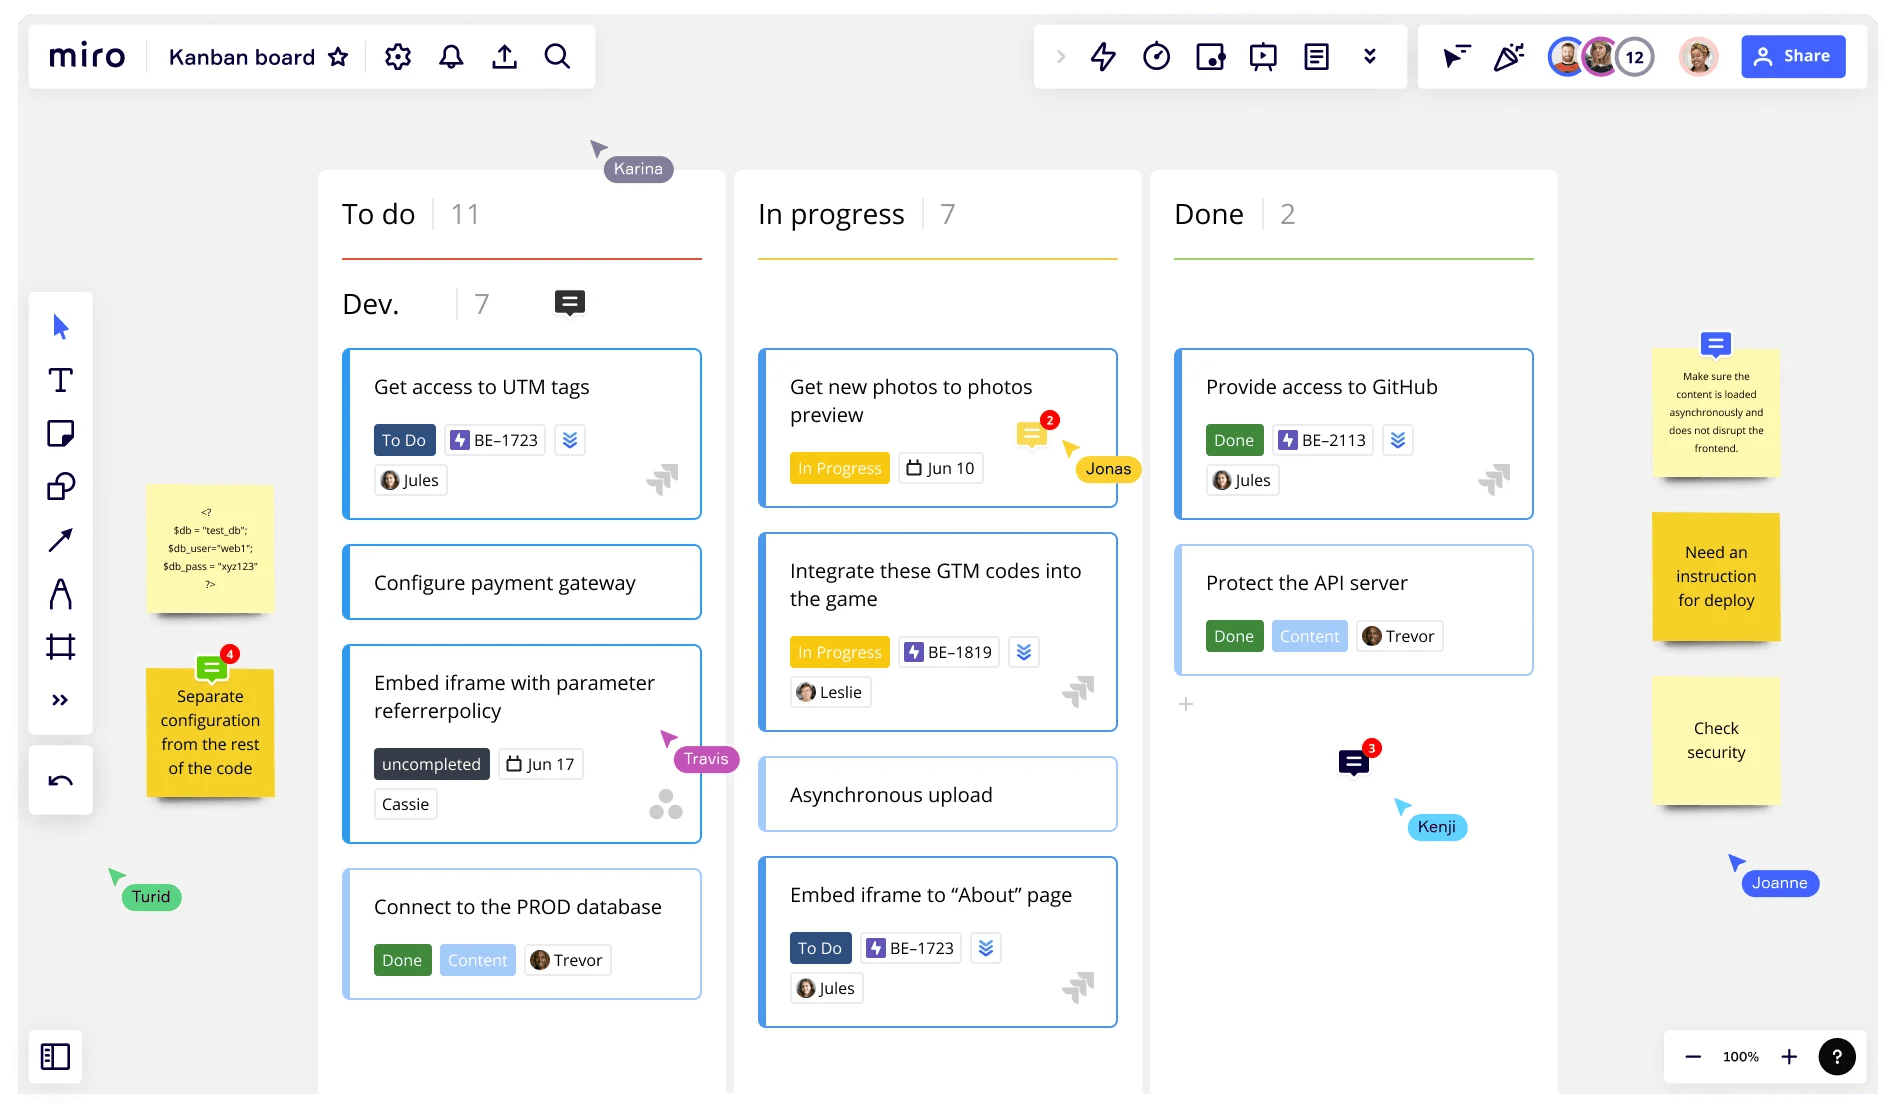
\includegraphics[width=0.9\textwidth]{assets/images/kanban-ejemplo.png}
\caption{Ejemplo básico de tablero Kanban con columnas, tarjetas, WIP y swimlanes.}
\end{figure}

Este ejemplo ilustra cómo la representación visual del trabajo facilita el seguimiento, la colaboración y la mejora continua.


\section{Fases del flujo de trabajo en Kanban}

En el contexto de Kanban, el \textbf{flujo de trabajo} representa la secuencia de pasos o estados por los que atraviesan las tareas desde que se conciben hasta que se completan. Este flujo no es rígido, sino que se adapta a las necesidades específicas de cada equipo o proceso organizacional. El objetivo es visualizar, gestionar y optimizar el flujo para garantizar una entrega continua de valor.

\subsection{Importancia del flujo de trabajo}

La visualización del flujo permite:
\begin{itemize}
    \item Identificar cuellos de botella y retrasos.
    \item Evaluar la eficiencia del proceso actual.
    \item Establecer límites de trabajo en curso (WIP) por fase.
    \item Mejorar continuamente el rendimiento del equipo.
\end{itemize}

Además, una representación clara del flujo facilita la comprensión compartida del proceso y promueve la colaboración entre los miembros del equipo.

\subsection{Fases comunes en un tablero Kanban}

Si bien cada implementación de Kanban puede diferir, muchas organizaciones adoptan una estructura de flujo que comprende las siguientes etapas:

\subsubsection{Backlog / Ideas / Por hacer (\textit{To Do})}

En esta fase se encuentran todas las tareas aún no iniciadas. Representa el conjunto de elementos que están listos para ser priorizados y ejecutados. Es habitual que se realicen sesiones de refinamiento para evaluar la viabilidad, esfuerzo requerido y prioridad de estas tareas.

\subsubsection{En progreso (\textit{Doing})}

Corresponde a las tareas que se encuentran activamente en desarrollo. Este estado refleja el trabajo que está siendo ejecutado por los miembros del equipo. Es recomendable que cada miembro se enfoque en una o pocas tareas a la vez para evitar la sobrecarga de trabajo y fomentar la finalización efectiva.

\subsubsection{Revisión / Pruebas / Validación}

Una vez completado el desarrollo inicial de una tarea, esta puede requerir validaciones adicionales. Dependiendo del tipo de proyecto, esta fase puede incluir:
\begin{itemize}
    \item Revisión de código
    \item Pruebas funcionales o de integración
    \item Verificación del cumplimiento de criterios de aceptación
    \item Evaluación por parte del cliente o partes interesadas
\end{itemize}

Esta etapa asegura la calidad antes de dar por finalizada la entrega.

\subsubsection{Hecho (\textit{Done})}

Representa la finalización formal de una tarea. Las tareas en esta columna han sido revisadas, validadas y están listas para su despliegue o ya han sido entregadas al cliente. Este estado implica cumplimiento total de los requisitos establecidos.

\subsection{Ejemplo de flujo de trabajo adaptado}

En un entorno de desarrollo de software, el flujo de trabajo podría incluir fases adicionales como:
\begin{itemize}
    \item Diseño UI/UX
    \item Aprobación del Product Owner
    \item Despliegue a producción
\end{itemize}

Por otro lado, en equipos de atención al cliente o marketing, las fases pueden ser completamente diferentes. Lo esencial es que el flujo refleje de forma precisa cómo se ejecuta el trabajo en el contexto real del equipo.

\subsection{Visualización de un flujo de trabajo típico}

\begin{figure}[H]
\centering
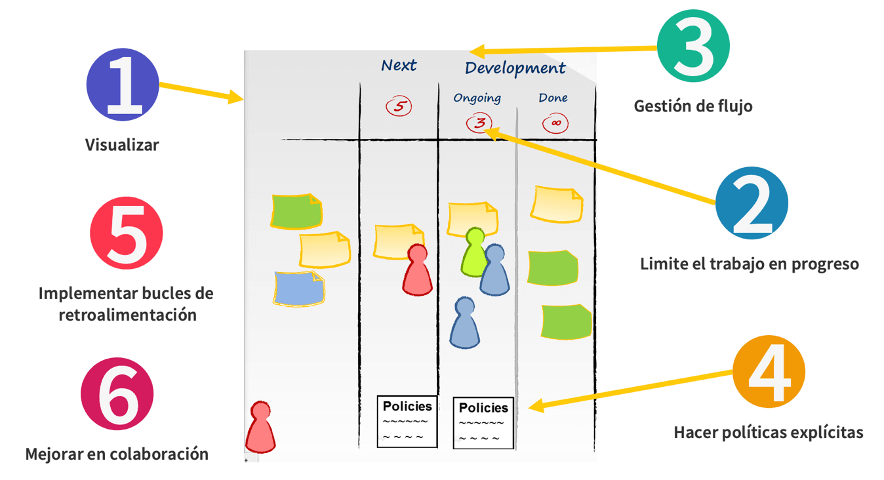
\includegraphics[width=0.9\textwidth]{images/flujo-kanban.png}
\caption{Ejemplo de un flujo de trabajo típico en un tablero Kanban.}
\end{figure}

Este ejemplo gráfico evidencia cómo se puede estructurar visualmente el recorrido de una tarea desde su planificación hasta su finalización.

\subsection{Consideraciones sobre la personalización del flujo}

Kanban no prescribe fases específicas ni impone un modelo único. De hecho, uno de sus principios fundamentales es adaptarse al flujo actual y evolucionarlo progresivamente. Esto significa que:
\begin{itemize}
    \item Cada equipo puede definir su propio flujo de trabajo.
    \item Las fases pueden cambiar con el tiempo conforme se detectan oportunidades de mejora.
    \item Se deben documentar y comunicar las políticas que regulan la transición entre fases.
\end{itemize}

La capacidad de adaptación es uno de los factores clave que diferencian a Kanban de otras metodologías ágiles más prescriptivas.


\section{Roles en Kanban}

A diferencia de otras metodologías ágiles como Scrum, Kanban no define de manera explícita roles formales o jerarquías dentro del equipo. Esta característica responde a su filosofía de mínima interrupción de los procesos existentes, enfocándose en la mejora continua a partir del flujo de trabajo actual.

\subsection{Enfoque general de los roles en Kanban}

En Kanban, todos los miembros del equipo son responsables del flujo de trabajo. No obstante, en la práctica, algunos roles pueden emerger de manera natural para facilitar la gestión y mejora del sistema. Estos roles, aunque no impuestos por la metodología, pueden aportar claridad, liderazgo y soporte al proceso.

\subsection{Roles emergentes comunes}
\begin{figure}[H]
    \centering
    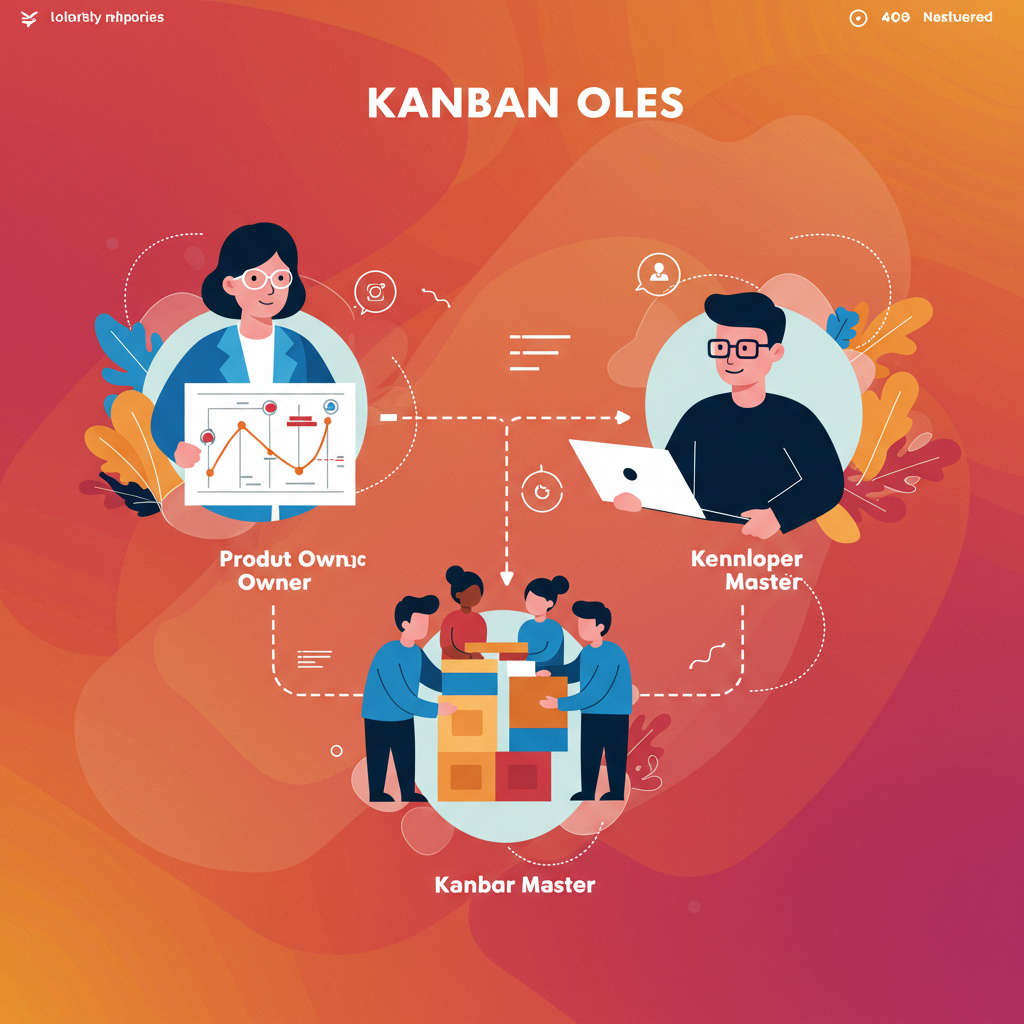
\includegraphics[width=0.6\textwidth]{assets/images/roles-kanban.png}
    \caption{Roles emergentes en Kanban y su relación con el flujo de trabajo}
    \label{fig:roles-kanban}
\end{figure}

A continuación, se describen los roles más comunes que suelen encontrarse en equipos que adoptan Kanban:

\subsubsection{Equipo de trabajo (Team Members)}

Son los responsables de ejecutar las tareas visibles en el tablero. Esto incluye desarrolladores, analistas, diseñadores u otros especialistas según el contexto del equipo. Cada miembro contribuye al cumplimiento de los objetivos colectivos y comparte la responsabilidad de mantener el flujo de trabajo en movimiento.

\subsubsection{Facilitador o Service Delivery Manager (SDM)}

Aunque no es un rol obligatorio, muchas organizaciones designan a una persona encargada de observar y optimizar el flujo. Su función se asemeja en cierta medida al \textit{Scrum Master}, aunque con un enfoque más operativo:
\begin{itemize}
    \item Detectar cuellos de botella
    \item Asegurar que los límites WIP se respeten
    \item Facilitar reuniones de mejora continua
    \item Promover la colaboración entre las partes interesadas
\end{itemize}

\subsubsection{Product Owner o Request Manager}

Cuando se trabaja en entornos con múltiples solicitudes externas, este rol emerge como intermediario entre los stakeholders y el equipo. Se encarga de priorizar las tareas, clarificar requerimientos y asegurar que el trabajo refleje el valor esperado por el cliente.

\subsection{Comparación con Scrum}

\begin{longtable}{|p{5cm}|p{5cm}|}
\hline
\textbf{Scrum} & \textbf{Kanban} \\
\hline
Scrum Master: facilitador y guía del proceso & Puede haber un Facilitador, pero no es obligatorio \\
\hline
Product Owner: responsable del valor del producto & Puede existir un Request Manager que prioriza el trabajo \\
\hline
Equipo de desarrollo: multifuncional y autogestionado & Equipo responsable del flujo, sin roles estrictos \\
\hline
Roles definidos y requeridos & Roles flexibles y emergentes según necesidad \\
\hline
\end{longtable}

\subsection{Responsabilidad compartida}

Una característica clave de Kanban es que todos los integrantes comparten la responsabilidad sobre:
\begin{itemize}
    \item El cumplimiento de los límites WIP
    \item La calidad del trabajo entregado
    \item La identificación de oportunidades de mejora
    \item La documentación de políticas y cambios en el flujo
\end{itemize}

Esto refuerza una cultura de colaboración constante y evolución adaptativa, que busca la eficiencia más allá de los roles individuales.


\section{Implementación de Kanban}

La implementación de Kanban en una organización requiere de una estrategia progresiva y adaptativa, en la cual se respeten los procesos existentes y se promueva una mejora continua sin generar disrupciones drásticas. Su adopción no demanda reorganización estructural ni la redefinición de roles, lo que lo convierte en una metodología accesible y flexible.

\subsection{Pasos para la adopción efectiva de Kanban}

Aunque no existe una única forma de implementar Kanban, se sugieren los siguientes pasos como guía inicial:

\subsubsection{1. Visualizar el trabajo actual}
El primer paso consiste en representar gráficamente el flujo de trabajo mediante un tablero Kanban. Se debe identificar:
\begin{itemize}
    \item Las etapas por las que transita una tarea desde su inicio hasta su entrega.
    \item Las tareas actuales en curso y pendientes.
    \item Responsables y tipos de trabajo.
\end{itemize}
Esto permite al equipo tener una visión clara del estado de cada tarea y detectar ineficiencias o cuellos de botella.

\subsubsection{2. Limitar el trabajo en curso (WIP)}
Establecer límites al número de tareas que pueden estar simultáneamente en una misma columna o etapa evita la sobrecarga del equipo y fomenta la finalización antes de iniciar nuevas actividades. Esta práctica mejora la eficiencia y reduce los tiempos de entrega.

\subsubsection{3. Gestionar y medir el flujo}
Una vez definido el flujo y aplicado el WIP, se deben monitorizar los tiempos de ciclo, la cantidad de tareas completadas por unidad de tiempo y la estabilidad del sistema. Esto permite tomar decisiones informadas para optimizar el rendimiento.

\subsubsection{4. Hacer las políticas explícitas}
Las reglas internas del equipo sobre cómo se prioriza, revisa o transfiere una tarea deben estar documentadas y visibles. Esto asegura la coherencia, promueve la transparencia y facilita la incorporación de nuevos miembros.

\subsubsection{5. Utilizar bucles de retroalimentación}
Se recomienda establecer momentos regulares para revisar el desempeño y discutir oportunidades de mejora. Algunas de las reuniones comunes en Kanban incluyen:
\begin{itemize}
    \item \textbf{Revisión diaria del tablero (Daily Kanban)}
    \item \textbf{Revisión de flujo de trabajo (Flow Review)}
    \item \textbf{Reunión de retrospectiva o mejora continua (Operations Review)}
\end{itemize}

\subsubsection{6. Mejorar de forma colaborativa y continua}
Kanban se basa en la mejora incremental. Las decisiones sobre cambios deben surgir de la observación colectiva y del análisis de datos, respetando el ritmo del equipo y los objetivos del sistema.

\subsection{Buenas prácticas para una implementación exitosa}

\begin{itemize}
    \item Iniciar con lo que ya se hace (sin imponer un nuevo proceso).
    \item Fomentar la participación activa de todos los miembros del equipo.
    \item Utilizar indicadores visuales para facilitar la comunicación.
    \item Mantener reuniones breves pero regulares para sincronizar avances.
    \item Capacitar al equipo en conceptos clave de flujo y mejora continua.
\end{itemize}

\subsection{Herramientas digitales para gestionar Kanban}

Existen múltiples plataformas que permiten digitalizar tableros Kanban y gestionar el flujo de trabajo en entornos colaborativos. Algunas de las más utilizadas incluyen:

\begin{itemize}
    \item \textbf{Trello:} Intuitiva, flexible y con múltiples integraciones.
    \item \textbf{Jira:} Ideal para equipos de desarrollo, con opciones de métricas y reportes avanzados.
    \item \textbf{Azure DevOps:} Integrada con repositorios de código y flujos CI/CD.
    \item \textbf{Kanbanize, ClickUp, Monday.com:} Alternativas empresariales con funciones de automatización.
\end{itemize}

Estas herramientas no solo facilitan la visualización del flujo de trabajo, sino también la recolección de métricas, la gestión de dependencias y la colaboración entre equipos distribuidos.


\section{Ventajas y desventajas de Kanban}

El enfoque Kanban, derivado de los principios Lean, ha demostrado ser una herramienta eficaz en la gestión de proyectos, especialmente en contextos donde la flexibilidad, la mejora continua y la visualización del trabajo son esenciales. No obstante, como toda metodología, presenta beneficios significativos, pero también limitaciones que deben ser consideradas al momento de su implementación.

\subsection{Ventajas de Kanban}

\begin{itemize}
    \item \textbf{Visualización clara del trabajo:} Uno de los mayores beneficios de Kanban es la representación gráfica del flujo de tareas, lo que permite al equipo identificar cuellos de botella, retrasos y sobrecarga de trabajo de forma inmediata.
    
    \item \textbf{Incremento en la eficiencia:} Al limitar el trabajo en curso (WIP) y promover el enfoque en tareas específicas, se reducen las interrupciones y se mejora el rendimiento general del equipo.
    
    \item \textbf{Adaptabilidad y flexibilidad:} A diferencia de metodologías como Scrum, Kanban no impone iteraciones fijas, por lo que es ideal para entornos con requerimientos cambiantes o impredecibles.
    
    \item \textbf{Mejora continua (Kaizen):} La retroalimentación constante, junto con la revisión de métricas del flujo, facilita procesos de mejora progresiva basados en datos reales y decisiones colaborativas.
    
    \item \textbf{Facilidad de adopción:} Kanban puede integrarse sin necesidad de reestructurar por completo la organización o redefinir roles, lo cual reduce la resistencia al cambio.
    
    \item \textbf{Mayor transparencia y alineación:} Al hacer visibles las políticas de trabajo, los estados de las tareas y los límites, se promueve una cultura de responsabilidad compartida y toma de decisiones consensuada.
\end{itemize}

\subsection{Desventajas de Kanban}

\begin{itemize}
    \item \textbf{Falta de estructura formal:} Al carecer de roles definidos y de ciclos de trabajo estrictos, Kanban puede resultar confuso para equipos que requieren dirección clara o estructuras más rígidas.
    
    \item \textbf{Dificultad para escalar:} Aunque se puede adaptar a contextos más amplios, Kanban no ofrece, de forma nativa, un marco completo para la gestión de múltiples equipos o grandes proyectos sin personalización adicional.
    
    \item \textbf{Riesgo de acumulación de tareas:} Si no se establecen y respetan correctamente los límites WIP, pueden generarse embudos de trabajo que comprometan el flujo y la calidad de las entregas.
    
    \item \textbf{Dependencia del compromiso del equipo:} El éxito de Kanban depende en gran medida de la disciplina y el compromiso del equipo para seguir las políticas, mantener actualizado el tablero y revisar el desempeño.
    
    \item \textbf{Menor visibilidad de largo plazo:} Al centrarse en el flujo continuo y no en entregas por iteraciones, puede dificultarse la planificación a mediano o largo plazo si no se combinan herramientas complementarias.
\end{itemize}

\subsection{Consideraciones finales}

La elección de Kanban como metodología de trabajo debe estar alineada con las necesidades, cultura y madurez del equipo. Sus beneficios se maximizan en contextos donde se valora la autonomía, la mejora progresiva y la adaptabilidad. No obstante, requiere un entorno colaborativo y comprometido para evitar caer en una gestión desorganizada o poco efectiva.


\section{Comparación con otras metodologías ágiles}

El ecosistema de metodologías ágiles ofrece diversos enfoques para la gestión eficiente de proyectos, cada uno con características particulares que los hacen más o menos adecuados según el tipo de equipo, producto o contexto organizacional. En esta sección se analiza comparativamente a Kanban frente a otras metodologías ágiles ampliamente utilizadas, tales como Scrum y eXtreme Programming (XP), resaltando similitudes, diferencias y ámbitos de aplicación.

\subsection{Kanban vs Scrum}

\textbf{Scrum} es probablemente la metodología ágil más difundida. Se estructura en ciclos temporales fijos denominados \textit{sprints}, que suelen tener una duración de entre 1 y 4 semanas. Incluye roles definidos (Scrum Master, Product Owner, equipo de desarrollo) y una serie de eventos obligatorios (Daily Scrum, Sprint Planning, Sprint Review, Sprint Retrospective).

Por el contrario, \textbf{Kanban} es menos prescriptivo y no impone iteraciones fijas ni roles formales. Se centra en el flujo continuo del trabajo y en la mejora progresiva basada en la visualización y medición del sistema actual.

\begin{itemize}
    \item \textbf{Estructura temporal:} Scrum trabaja en bloques temporales cerrados; Kanban es continuo y flexible.
    \item \textbf{Roles:} Scrum define roles estrictos; Kanban los deja abiertos según el contexto.
    \item \textbf{Planeación:} Scrum realiza una planificación exhaustiva al inicio del sprint; Kanban permite añadir y priorizar tareas de forma dinámica.
    \item \textbf{Adaptabilidad:} Kanban es más adecuado cuando los requisitos cambian constantemente; Scrum funciona mejor con requisitos más estables por iteración.
\end{itemize}

\subsection{Kanban vs eXtreme Programming (XP)}

\textbf{XP (eXtreme Programming)} es una metodología enfocada en mejorar la calidad del software mediante prácticas técnicas rigurosas como programación en pareja, desarrollo guiado por pruebas (TDD) y entrega continua. A diferencia de Kanban, XP está fuertemente ligado al ámbito técnico y al desarrollo de software como actividad central.

\begin{itemize}
    \item \textbf{Enfoque técnico:} XP es intensamente técnico; Kanban es más general y aplicable a múltiples dominios.
    \item \textbf{Prácticas:} XP prescribe un conjunto de buenas prácticas específicas; Kanban ofrece principios adaptables al contexto.
    \item \textbf{Flexibilidad:} Kanban permite introducir mejoras de forma progresiva sin grandes cambios iniciales; XP requiere el compromiso con sus prácticas desde el inicio.
\end{itemize}

\subsection{¿Cuándo usar Kanban?}

Kanban es especialmente recomendable en los siguientes escenarios:

\begin{itemize}
    \item Cuando los requerimientos cambian frecuentemente y no es posible planificar con anticipación mediante iteraciones cerradas.
    \item En equipos que ya cuentan con un proceso de trabajo, pero desean introducir mejoras progresivas sin rupturas.
    \item En proyectos de soporte, mantenimiento, atención al cliente u operaciones, donde el flujo continuo es prioritario.
    \item Cuando se busca una transición hacia un modelo ágil sin una reestructuración profunda del equipo o proceso actual.
\end{itemize}

\subsection{Síntesis comparativa}

\begin{longtable}{|p{4cm}|p{4.5cm}|p{4.5cm}|}
\hline
\textbf{Criterio} & \textbf{Scrum} & \textbf{Kanban} \\
\hline
Estructura & Iteraciones fijas (sprints) & Flujo continuo \\
\hline
Roles & Definidos y obligatorios & No prescriptivo \\
\hline
Planificación & Por sprint & Adaptativa y continua \\
\hline
Cambio de tareas & Limitado por sprint & Permitido en cualquier momento \\
\hline
Aptitud para cambios frecuentes & Media & Alta \\
\hline
Curva de aprendizaje & Alta & Baja \\
\hline
Ámbito técnico & Moderado & Amplio y general \\
\hline
\end{longtable}


\section{Casos de estudio o ejemplos prácticos}

La aplicación de la metodología Kanban ha trascendido el ámbito del desarrollo de software, extendiéndose con éxito a diversos sectores industriales y de servicios. En esta sección se presentan ejemplos prácticos que evidencian cómo la implementación de Kanban ha contribuido a mejorar la eficiencia operativa, optimizar flujos de trabajo y fomentar una cultura de mejora continua.

\subsection{Caso 1: Desarrollo de software en una startup tecnológica}

Una startup dedicada al desarrollo de aplicaciones móviles adoptó Kanban para gestionar su proceso de desarrollo. Inicialmente, el equipo enfrentaba problemas como sobrecarga de tareas, falta de visibilidad sobre el estado del proyecto y retrasos recurrentes en las entregas.

\begin{itemize}
    \item \textbf{Acciones implementadas:} se diseñó un tablero Kanban digital con columnas como \textit{To Do}, \textit{En Progreso}, \textit{En Pruebas} y \textit{Terminado}. Se establecieron límites WIP y se realizaron reuniones semanales de revisión de flujo.
    \item \textbf{Resultados:} en tres meses, se redujo el tiempo promedio de entrega de funcionalidades en un 40\%, se detectaron cuellos de botella en la etapa de pruebas y se mejoró la colaboración entre los desarrolladores y el área de control de calidad.
\end{itemize}

\subsection{Caso 2: Atención al cliente en una empresa de telecomunicaciones}

Una empresa nacional de telecomunicaciones incorporó Kanban en su centro de atención al cliente con el objetivo de mejorar la gestión de incidencias técnicas reportadas por usuarios.

\begin{itemize}
    \item \textbf{Acciones implementadas:} el equipo utilizó un tablero físico que representaba cada etapa del proceso de resolución de incidentes (Recepción, Diagnóstico, Solución, Cierre). Se asignaron responsables visibles en cada tarea y se midieron los tiempos de resolución promedio.
    \item \textbf{Resultados:} la tasa de resolución en primera llamada aumentó un 25\%, mientras que los tiempos de atención bajaron de 48 a 28 horas en promedio. Además, se logró una mayor transparencia en la carga de trabajo de cada agente.
\end{itemize}

\subsection{Caso 3: Gestión de marketing digital}

Un equipo de marketing de una agencia publicitaria decidió aplicar Kanban para gestionar sus campañas publicitarias en redes sociales. Antes de la implementación, los plazos de entrega eran poco predecibles y las tareas se acumulaban en la etapa de diseño gráfico.

\begin{itemize}
    \item \textbf{Acciones implementadas:} el tablero incluyó columnas específicas como \textit{Brief recibido}, \textit{Diseño en proceso}, \textit{Revisión del cliente}, \textit{Programado} y \textit{Publicado}. Se colocaron límites WIP y se priorizaron tareas urgentes con tarjetas de color.
    \item \textbf{Resultados:} se logró una planificación más precisa de publicaciones semanales, el equipo de diseño redujo el tiempo de respuesta en un 30\% y se minimizó la duplicación de esfuerzos.
\end{itemize}

\subsection{Análisis transversal de los casos}

Los tres casos anteriores demuestran que Kanban puede adaptarse a diversos contextos organizacionales, siempre que se respete el principio de visualizar el trabajo, gestionar el flujo y aplicar mejoras de forma incremental. Entre los beneficios observados se destacan:

\begin{itemize}
    \item Aumento de la eficiencia y visibilidad del proceso.
    \item Identificación de cuellos de botella.
    \item Mayor responsabilidad compartida y autonomía del equipo.
    \item Flexibilidad frente a cambios inesperados o tareas urgentes.
\end{itemize}

Estos resultados refuerzan la utilidad de Kanban como metodología versátil y de bajo costo de adopción para entornos que requieren adaptabilidad, colaboración y mejora continua.


\section{Conclusiones}

El presente informe ha permitido realizar un análisis riguroso, detallado y multidimensional de la metodología ágil Kanban, desde sus orígenes industriales hasta su consolidación como herramienta estratégica en la gestión de proyectos y equipos de trabajo. A través de la investigación y el estudio de casos reales, se ha demostrado que Kanban no solo es una técnica visual de organización, sino una filosofía de mejora continua orientada a la eficiencia operativa y la transparencia colaborativa.

En primer lugar, la comprensión de los principios fundamentales de Kanban —como la visualización del flujo de trabajo, la limitación del trabajo en curso (WIP) y el fomento de ciclos de retroalimentación— permite al equipo adoptar prácticas de gestión adaptativas y menos prescriptivas que otras metodologías ágiles. Este enfoque, al centrarse en la evolución progresiva y no en revoluciones estructurales, facilita su adopción incluso en organizaciones con escasa experiencia previa en agilidad.

Asimismo, el desglose del flujo de trabajo en fases claras, acompañado del uso de tableros físicos o digitales, ha demostrado su eficacia en sectores tan diversos como el desarrollo de software, la atención al cliente y la gestión de campañas publicitarias. Esta adaptabilidad subraya la naturaleza versátil de Kanban, la cual lo hace apto tanto para entornos dinámicos como para contextos donde se requiere una estructura más estable.

Otro aspecto destacable es la flexibilidad de roles y la ausencia de jerarquías rígidas, lo cual empodera a los miembros del equipo, promueve la autorregulación y fortalece la colaboración horizontal. No obstante, la correcta implementación de Kanban exige un compromiso organizacional con la transparencia, el análisis continuo de cuellos de botella y la disposición para ajustar procesos sobre la marcha.

En términos comparativos, Kanban se diferencia de metodologías como Scrum por su enfoque evolutivo, lo cual lo convierte en una alternativa viable para equipos que requieren un modelo de transición más suave hacia la agilidad.

Finalmente, esta investigación grupal nos ha permitido consolidar un aprendizaje integral no solo sobre la técnica en sí, sino también sobre el valor de trabajar colaborativamente, analizar fuentes académicas de calidad y plasmar conocimientos de forma estructurada y crítica. En un entorno académico y profesional cada vez más orientado a la adaptabilidad y la eficiencia, dominar herramientas como Kanban representa una competencia clave para los futuros ingenieros de software.

\section*{Glosario de términos}

A continuación, se presenta un glosario con términos clave utilizados a lo largo del informe, con el fin de facilitar la comprensión del lector:

\begin{description}
    \item[Agilidad:] Capacidad de una organización o equipo para adaptarse rápidamente a cambios, entregar valor de forma continua y responder con flexibilidad ante nuevas necesidades.
    
    \item[Backlog:] Lista priorizada de tareas, funcionalidades o elementos de trabajo pendientes por desarrollar o ejecutar dentro de un proyecto.
    
    \item[Flujo de trabajo (Workflow):] Conjunto de etapas o pasos secuenciales que sigue una tarea desde su inicio hasta su finalización.
    
    \item[Kaizen:] Término japonés que significa “mejora continua”. En Kanban, hace referencia a la práctica constante de identificar y aplicar pequeñas mejoras para optimizar procesos.
    
    \item[Kanban:] Metodología ágil de gestión visual del trabajo basada en principios del Lean Manufacturing, que promueve la eficiencia, transparencia y mejora continua en la entrega de valor.
    
    \item[Límites WIP (Work In Progress):] Restricciones impuestas al número de tareas que pueden estar en proceso simultáneamente, con el fin de evitar sobrecarga y mejorar el flujo.
    
    \item[Lean Manufacturing:] Filosofía de gestión enfocada en la eliminación de desperdicios, mejora continua y entrega eficiente de valor al cliente.
    
    \item[Scrum:] Marco de trabajo ágil basado en iteraciones cortas llamadas sprints, con roles definidos y reuniones periódicas para planificar, revisar y ajustar el trabajo.
    
    \item[Swimlanes:] Divisiones horizontales en un tablero Kanban que agrupan tareas por tipo, responsable, prioridad u otro criterio relevante.
    
    \item[Tarjeta Kanban:] Representación visual de una tarea o unidad de trabajo. Contiene información clave como el nombre de la tarea, responsable, fecha de entrega, entre otros.
    
    \item[Visualización:] Principio fundamental de Kanban que implica representar gráficamente el trabajo para facilitar su seguimiento, priorización y toma de decisiones.
\end{description}

\vspace{0.5cm}

\noindent\textbf{Palabras clave:} Kanban, mejora continua, flujo de trabajo, Lean, tablero Kanban, visualización, límites WIP, agilidad, gestión de proyectos, eficiencia.

\section{Bibliografía}

\begin{itemize}
    \item Ahmad, M. O., Markkula, J., \& Oivo, M. (2021). Kanban in software engineering: A systematic mapping study. \textit{Journal of Systems and Software}, 181, 111028. https://doi.org/10.1016/j.jss.2021.111028

    \item Corona, E., \& Pani, F. E. (2020). A review of lean–kanban approaches in software development. \textit{Journal of Software: Evolution and Process}, 32(1), e2207. https://doi.org/10.1002/smr.2207

    \item González, P., \& Jiménez, S. (2023). Aplicación de metodologías ágiles: Un enfoque práctico de Kanban en proyectos tecnológicos. \textit{Revista Latinoamericana de Ingeniería de Software}, 5(2), 45-59.

    \item Sutherland, J., \& Schwaber, K. (2020). \textit{The Scrum Guide}. Scrum.org. Recuperado de \url{https://scrumguides.org/}

    \item Martínez, A., \& López, R. (2022). Kanban como estrategia para la mejora del flujo de trabajo en organizaciones ágiles. \textit{Revista Iberoamericana de Gestión de Proyectos}, 11(1), 33-48. https://doi.org/10.31039/ijocs.2022.11.1.3

    \item Project Management Institute. (2021). \textit{Guía de los Fundamentos para la Dirección de Proyectos (Guía del PMBOK)} (7ª ed.). Project Management Institute.

    \item Kniberg, H. (2022). \textit{Kanban and Scrum: How to Make the Most of Both} (2ª ed.). C4Media.
\end{itemize}



\end{document}
